<<<<<<< HEAD
Compressed sensing (CS) has one of the topics that attracted a lot of interests over the past years. Suppose $z$ is a length-$N$ signal. It is said to be $S$-sparse(or compressible) if $z$ can be well approximated using only $S << N$ coefficients under some linear transformation
$ z=\Psi x $
where $\Psi$ is the sparsifying basis and $x$ is transform coefficient vector that has at most $S$(significant) nonzero entries.
\\

The Basis pursuit problem 
\begin{equation}
\min ||x||_{l_1} \quad \text{ subject to } \quad \Phi \Psi x=y
\end{equation}


Where $\Psi$ is an $n \times n$ orthogonal matrix corresponding to the basis in which our signal $z = \Psi x$ is $S$-sparse. $\Phi$ is our sensing matrix. 
\\
\subsection*{Structured matrix}
\textbf{Toeplitz} and \textbf{Circulant} matrices have the forms, respectively,
\\

$$
T = \begin{bmatrix}
t_{1}    & t_{2}    & ...    & t_{n}   \\[0.3em]
t_{n+1}  & t_{1}    & ...    & t_{n-1} \\[0.3em]
\ddots   & \ddots   & \ddots &         \\[0.3em]
t_{2n-1} & t_{2n-2} & ...    & t_{1}         
\end{bmatrix}
\qquad \text{and} \qquad
C = \begin{bmatrix}
t_{1}  & t_{2}  & ...    & t_{n}   \\[0.3em]
t_{n}  & t_{1}  & ...    & t_{n-1} \\[0.3em]
\ddots & \ddots & \ddots &         \\[0.3em]
t_{2}  & t_{3}  & ...    & t_{1}        
\end{bmatrix} 
$$
\\
	Any Circulant matrix can be diagonalized by a Fourier transform, i.e. obeying
	$$ C=\frac{1}{\sqrt{n}} F^* \Sigma F $$ with $F$ as the discrete Fourier matrix
	$F_{t,w}=e^{-i\; 2\pi(t-1)(w-1)/n}, \qquad 1 \le t,w \le n$
	$$
	\Sigma = \begin{bmatrix}
	\sigma_{1} & 0 & ...& 0           \\[0.3em]
	0 & \sigma_{2} & ... & 0 \\[0.3em]
	\ddots &\ddots & \ddots &      \\[0.3em]
	0 & 0 & ... & \sigma_{n}        
	\end{bmatrix} $$
	a diagonal matrix whose entries are unit magnitude complex numbers with random phases.
\\
	We generate $\sigma_{w}$ as follows:
	\\[1em]
	
	$w=1\qquad \qquad \qquad : \; \sigma_{1} \sim \pm$ 1 with equal probability,
	\\[1em]
	$2 \le w < n/2+1 \; \; : \; \sigma_{w}=e^{i\theta w}, where \; {\theta}_{w} \sim Uniform(0,2\pi) $
	\\[1em]
	$w=n/2+1 \qquad \; \; \, : \; \sigma_{n/2+1} \sim \pm 1 $ with equal probability 
	\\[1em]
	
	$n/2+2 \le w \le n \; \; : \; \sigma_{w}=\sigma^{*}_{n-w+2}$, conjugate of  $\sigma_{n-w+2}$.
	
	$$
	$$
	Generating the diagonal in this way ensures the resulting circulant matrix is real-valued due 
	to conjugate symmetry.
	$$
	T_{n} = \left[ \: 
	\begin{array}{*{4}{c}}
	\cline{1-4}
	\multicolumn{1}{|c}{t_{1}} & t_{2} & ...& \multicolumn{1}{c|}{t_{n}}           \\[0.3em]
	\cline{1-4}
	t_{n+1} & t_{1} & ... & t_{n-1} \\[0.3em]
	\ddots &\ddots & \ddots &    \\[0.3em]
	t_{2n-1} & t_{2n-2} & ... & t_{1}      \\[0.3em]    
	\end{array}
	\right]
	=
	\left[ \:
	\begin{array}{*{4}{c}}
	t_{1} & t_{2} & ...& t_{n}        \\[0.3em]
	\cline{1-1}
	\multicolumn{1}{|c|}{t_{n+1}} & t_{1} & ... & t_{n-1} \\[0.3em]
	\multicolumn{1}{|c|}{\ddots} & \ddots & \ddots &    \\[0.3em]
	\multicolumn{1}{|c|}{t_{2n-1}} & t_{2n-2} & ... & t_{1}          \\[0.3em]
	\cline{1-1}
	\end{array}
	\right]
	$$
	\\
	$$
	C_{2n} =\begin{bmatrix}
	t_{1}   & t_{2} & ...    & t_{n}  & 0   & t_{2n-1} & ... &  t_{n+1}   \\[0.3em]
	t_{n+1} & t_{1} & ...    & t_{n-1}& ... & 0  & ... &          \\[0.3em]
	\ddots  &       & \ddots &        & \ddots & & &\ddots    \\[0.3em]
	\cdots  &       & \cdots &       & \cdots & & & \cdots
	\end{bmatrix}
	=
	\begin{bmatrix}
	T_{n} & B_{n}            \\[0.3em]
	B_{n} & T_{n}   
	\end{bmatrix}
	$$
	
	\textbf{Hadamard} matrix is a square matrix whose entries are either $+1$ or $-1$ and whose rows are mutually orthogonal.
\begin{figure}[h]
\centering
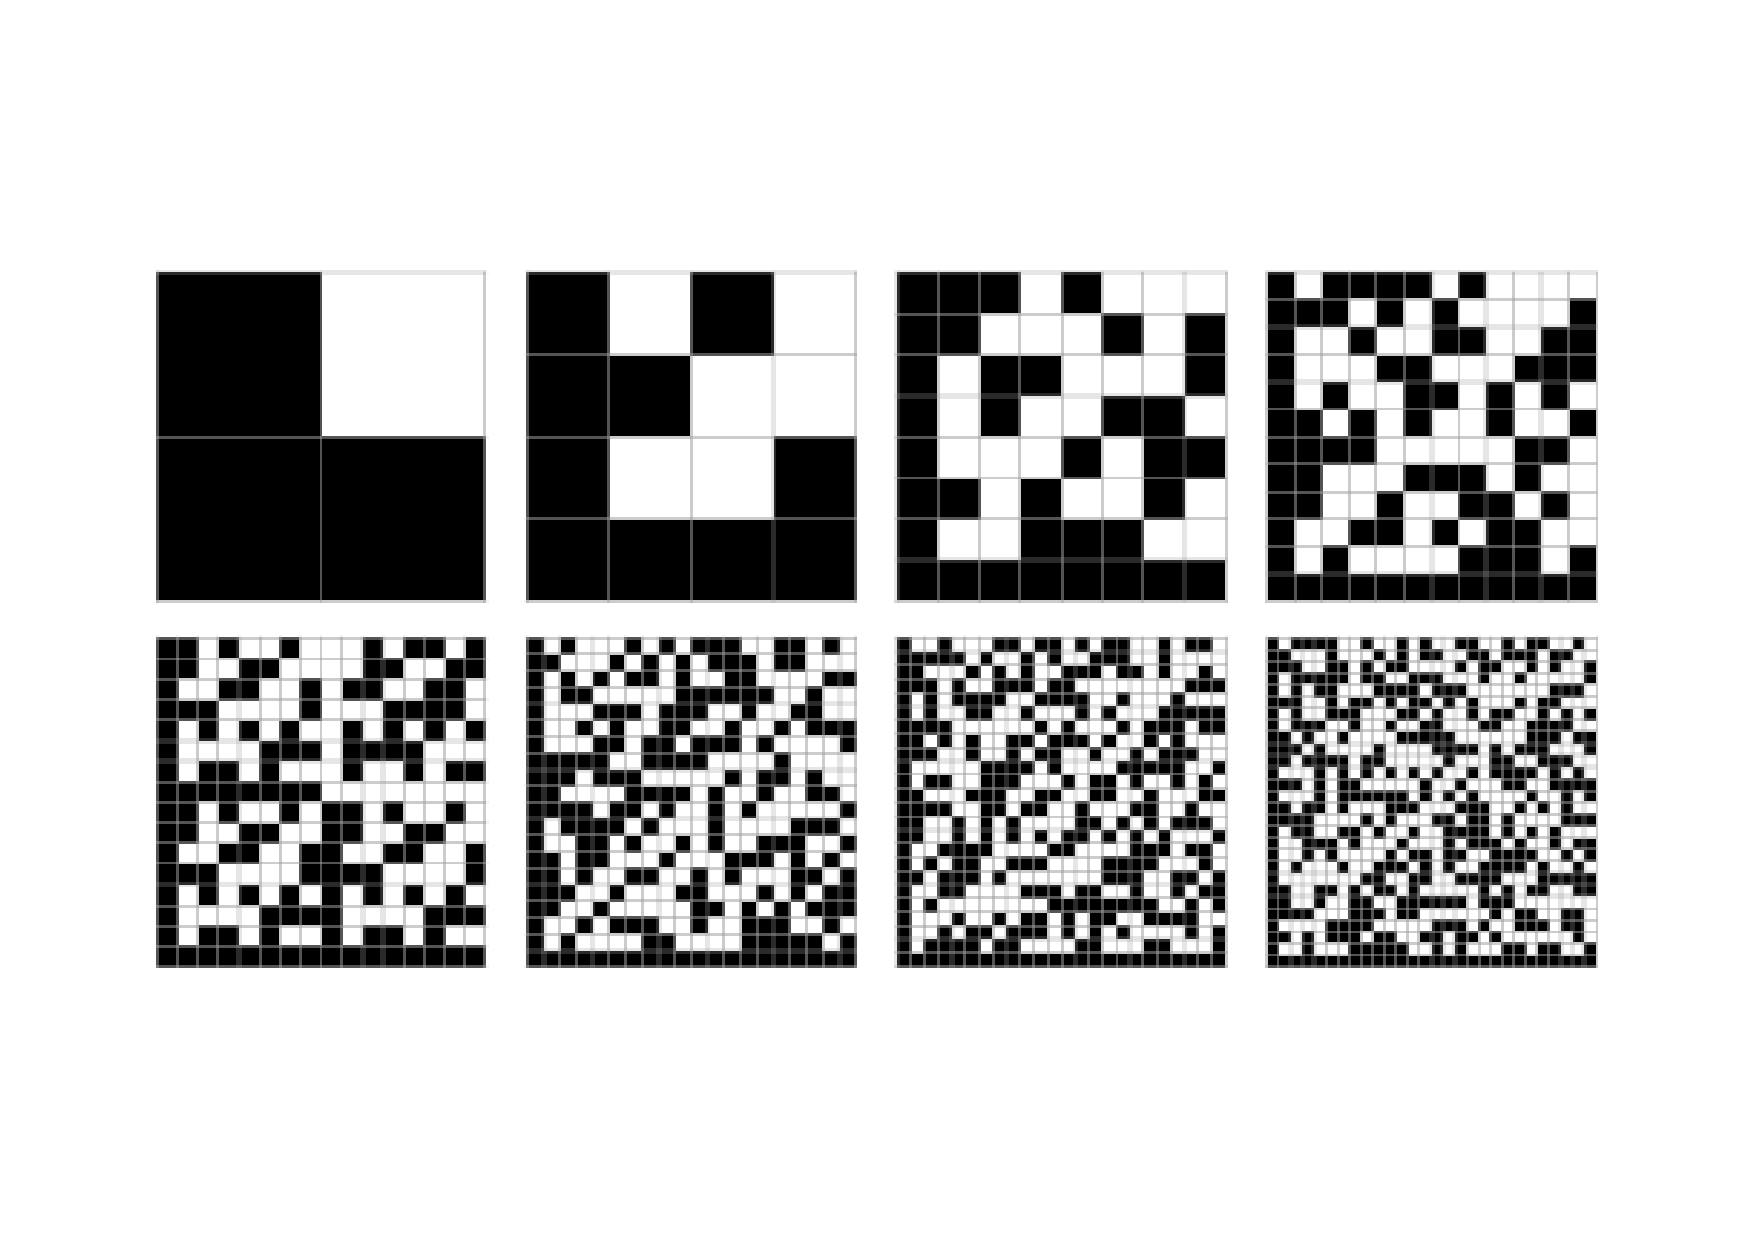
\includegraphics[width=0.7\linewidth]{HadamardMatrices_800}
\caption{}
\label{fig:HadamardMatrices_800}
\end{figure}


	An equivalent definition of the Hadamard matrices is given by 
	$$ H_{n} H_{n}^T = n  I_{n} $$
	where $I_{n}$ is the $n \times n$ identity matrix.
	$$
	H_{1} = \begin{bmatrix}
	1
	\end{bmatrix}
	\qquad
	H_{2} = \begin{bmatrix}
	1 & 1           \\[0.3em]
	1& -1
	\end{bmatrix}	
	\qquad
	H_{4} = \begin{bmatrix}
	H_{2} & H_{2}           \\[0.3em]
	H_{2}& -H_{2}
	\end{bmatrix}	
	$$
	$$
	\centering
	\qquad
	H_{2^{n}} = \begin{bmatrix}
	H_{2^{n-1}} & H_{2^{n-1}}           \\[0.3em]
	H_{2^{n-1}}& -H_{2^{n-1}}            
	\end{bmatrix}	
	$$





